% !TeX encoding = UTF-8

%===============================================================================
% Font options are:
%   plain (default), serif (uses Palladio), sans-serif (uses Paratype Sans)
% Layout options are:
%   article (default, no chapters), book (for longer texts, offers \chapter)
% Paragraph options are:
%   noparskip (default, no spacing between paragraphs), parskip (spaced)
\documentclass[serif,article,parskip]{agse-thesis}
\usepackage[font={small,it}]{caption}
\renewcommand{\baselinestretch}{1.5}

% Global parameters, replace with actual values.
\newcommand{\thesisTitle}{Traumapädagogik - wann und wozu und wann nicht mehr?}
\newcommand{\thesisSubtitle}{Zur Attraktivität des \textit{Traumas} für die Pädagogik}
% -> You may use \par (but not \\) to format the title. If you do so, you'll
%    need to manually set the 'pdftitle' attribute below.
\newcommand{\studentName}{Olga Urbaniak}
%===============================================================================

\hypersetup{pdftitle={\thesisTitle}}
\hypersetup{pdfauthor={\studentName}}

% Blind texts, for demonstration only, not part of the actual template
\usepackage{lipsum}

\begin{document}

\coverpage[
    student/id=1234567,
    student/mail=olga.urbaniak@fu-berlin.de,
    thesis/type=Bachelorarbeit,            % optional, default: Bachelorarbeit
    thesis/group={Arbeitsgruppe Software Engineering},
                                           % optional, default: AGSE
    thesis/firstAdvisor={1. Gutachterin: Prof. Dr. Ulrike Urban-Stahl},            thesis/secondAdvisor={2. Gutachterin: Prof. Dr. Katrin Kaufmann},           % optional
    thesis/examiner={Prof. Dr. Mia Maus},
    thesis/examiner/2={Prof. Dr. Bob Bär}, % optional
    thesis/date=\today,                    % optional, default: \today
   %title/size=\LARGE,      % set this value to overwrite automatic font size
   %abstract/separate       % toggle this to move the abstract to its own page
]

\clearpage
\tableofcontents

\clearpage
\listoffigures

\clearpage
\mainmatter
\setcounter{secnumdepth}{0}
% !TeX encoding = UTF-8
\section{Einführung}

Traumapädagogik bezeichnet eine junge Bewegung, die mit lebensgeschichtlich belasteten Kindern und Jugendlichen arbeitende Fachkräfte unterstützt (vgl. Weiß u. a., 2016: 11). Sie ist als Antwort auf die Überforderung der pädagogischen Praxis mit traumatisierten Kindern und Jugendlichen entstanden (vgl. Kühn 2014: 25). In den letzten Jahren entwickelte sich Traumapädagogik von vereinzelten Konzepten hin zu einer institutionalisierten Form mit eigenen Gremien, Zertifizierungen und Standards (vgl. Schimmer 2016: 439 ff.). Entstanden in der stationären Jugendhilfe, öffnet sich Traumapädagogik für andere pädagogische Arbeitsfelder, etwa Primarerziehung, Bildung und Behindertenhilfe als Bereiche, für die psychotraumatologisches Wissen bedeutsam ist (vgl. Bausum u. a. 2013: 8).

Trauma ist ein aus der Medizin stammender Begriff, der erst in den 1960er-Jahren seine psychiatrisch-psychologische Bedeutung einer psychischen Verletzung erhalten hat (vgl. Anhorn \& Balzereit 2016: 37). Trauma für sich ist keine Diagnose im Sinne einer psychischen Störung (vgl. ebd.), ebenso kein pädagogischer Begriff (vgl. Zimmermann 2016: 47). Dennoch ist sie zu einem so attraktiven Begriff für die pädagogische Praxis geworden, dass sich aus dieser Verbindung eine „eigenständige Fachrichtung“ (vgl. z. B. Bausum u. a. 2013: 8) entwickelt.

Die vorliegende Arbeit beschäftigt sich mit dem Phänomen der Traumapädagogik und geht der Frage nach, ob die pädagogische Praxis einer Traumapädagogik bedürfe. Wann und wozu und wann nicht mehr? Macht der Zugriff auf \textit{Trauma} die pädagogische Praxis handlungsfähiger?

Um sich den Antworten auf diese Fragen zu nähern, wird zunächst erklärt, was Traumapädagogik ist. Eine eindeutige Definition für diese noch junge und heterogene Bewegung gibt es (noch) nicht. Da \textit{Trauma} semantisch und inhaltlich zur Traumapädagogik gehört, die sich wiederum explizit auf die Psychotraumatologie bezieht, wird im ersten Kapitel der Traumabegriff erklärt. Auf dieser Grundlage werden die Entstehung und Institutionalisierung der „neuen Fachdisziplin“ nachverfolgt. Sind diese Hintergründe geklärt, wird im zweiten Kapitel der Blick frei, um sich mit der in der Traumapädagogik geforderten Haltung, den Inhalten der Konzepte sowie mit Traumapädagogik als institutionellem Konzept auseinanderzusetzen. Der Frage, warum es einer Traumapädagogik bedürfe, widmet sich das dritte Kapitel. Dabei sollen die Argumente für die Traumapädagogik, die in der Literatur zu finden sind, gesammelt werden. Das vierte Kapitel reflektiert kritisch das Vorangegangene und untersucht, wofür die Traumapädagogik benutzt wird. Dabei wird sichtbar, dass Traumapädagogik neue Probleme und Fragen generiert. Anschließend wird der Begriff \textit{Traumapädagogik} kritisch hinterfragt, um noch einmal die Frage nach dem Nutzen des \textit{Traumas} für die pädagogische Praxis anders zu stellen.


\setcounter{secnumdepth}{2}
% !TeX encoding = UTF-8
\section{Begriffliche Annäherung}

Der Begriff \textit{Trauma} entstammt dem Griechischen und bedeutet \textit{Wunde} oder \textit{Verletzung} (vgl. Landolt \& Hensel 2008: 14). Dabei wird nicht unterschieden, ob der Körper oder die Seele betroffen ist (vgl. ebd.). Folgendes Kapitel stellt eine erste Annährung an die Beantwortung der Frage dar, was Traumapädagogik sei. Dazu ist der Begriff \textit{Trauma} zu erklären (1.1), was nicht eindeutig möglich ist. Danach werden die in der Literatur vorfindlichen Definitionen der Traumapädagogik vorgestellt (1.2.). Das Kapitel schließt, indem die Entstehung und Institutionalisierung der Traumapädagogik beschrieben werden (1.3).

\subsection{Trauma}
Trauma ist ein Begriff, der in den letzten Jahren sowohl im Alltagsgebrauch als auch in verschiedenen psychosozialen Handlungsfeldern sehr populär geworden ist. Im allgemeinen Sprachgebrauch wird unter Traumatisierung meist eine seelische Verletzung verstanden (vgl. Hantke \& Görges 2012: 53). Der Begriff wird selbst in der Traumaforschung nicht eindeutig benutzt. Nicht immer wird deutlich, ob Trauma das Ereignis, die Auswirkungen, die Symptome oder das Leiden bedeutet (vgl. ebd). Die International Classification of Diseases (Internationale statistische Klassifikation der Krankheiten und verwandter Gesundheitsprobleme, kurz ICD, momentan gültige Fassung: ICD-10) definiert Trauma indirekt als ein „Ereignis oder eine Situation kürzerer oder längerer Dauer, mit außergewöhnlicher Bedrohung oder katastrophenartigem Ausmaß, die bei fast jedem eine tiefe Verzweiflung hervorrufen würde“ (ICD-10-GM 2016, F43.1). Im Diagnostic and Statistical Manual of Mental Disorders (zu Deutsch: Diagnostischer und statistischer Leitfaden psychischer Störungen, Fassung DSM-IV-TR) werden zwei Aspekte genannt, die gleichzeitig erfüllt werden müssen, um von Trauma zu sprechen: (1) das Erleben oder Beobachten eines Ereignisses, das eine ernsthafte Bedrohung der körperlichen oder psychischen Integrität der eigenen oder anderer Personen darstellt; (2) die Reaktionen der betroffenen Person sind von intensiver Furcht, Hilflosigkeit, Grauen und durch aufgelöstes oder agitiertes Verhalten begleitet (vgl. Saß u. a. 2003: 512). Im aktuellsten DSM V entfällt das zweite Kriterium, das sich auf das subjektive Erleben bezieht (vgl. Falkai u. a. 2015: 1111). Mit der Entstehung, der Erfassung, dem Verlauf und der Behandlung der Folgen lebensbedrohlicher und/oder extrem belastender Ereignisse befasst sich Psychotraumatologie (vgl. Landolt \& Hensel 2008: 14), die mit ihrer stressbezogenen Sichtweise (vgl. Hensel 2014: 27) von einem kausalen Zusammenhang zwischen dem Entstehen einer psychischen Störung und belastenden Lebensereignissen ausgeht. Laut Hausmann (2006: 16) beschäftigt sich Psychotraumatologie mit traumatischen Ereignissen und ihren Auswirkungen auf das Erleben und Verhalten von Einzelpersonen und sozialen Systemen. Ein psychisches Trauma sei dabei als ein zumeist plötzlich auftretendes Ereignis zu verstehen, das auf den Betroffenen sehr bedrohlich wirke und zugleich als nicht zu bewältigen erscheine (vgl. Hausmann 2006: 31). Ein Trauma löst intensive Gefühle des Ausgeliefertseins, der Hilflosigkeit, des Entsetzens, der Angst, Verzweiflung oder Wut aus oder führt zu einem Zustand der emotionalen Betäubung und Apathie. Ein psychisches Trauma kann langfristige psychische Symptome verursachen. Die traumatisierende Wirkung eines Ereignisses hängt von der Art des Geschehens sowie von dessen Umständen ab, aber auch von der betroffenen Person, ihren Handlungs- und Bewältigungsmöglichkeiten sowie verschiedenen Schutz- und Risikofaktoren (vgl. ebd.). Die Schutzfaktoren, die unter die Resilienz subsumiert werden und die die Auswirkungen der traumatischen Situationen abschwächen würden, verlieren laut Hensel an Bedeutung, je intensiver und häufiger die Belastung ist (vgl. Hensel 2014: 27). Die klassischen Diagnosen der Anpassungsstörung sowie die posttraumatische Belastungsstörung (PTBS) sind nicht die einzigen und häufigsten Folgen einer Traumatisierung (vgl. ebd.), obwohl hauptsächlich diese zur Verfügung stehen. Zu den typischen PTBS-Symptomen gehören, die traumatischen Erlebnisse in Form von Bildern, Gedanken, Wahrnehmungen oder Halluzinationen (sog. \textit{Flashbacks}) wiederholt zu erleben; mit dem Trauma verbundene Reize zu vermeiden; übertriebene Wachsamkeit. Fehlen diese Symptome, ist dies jedoch keine Garantie dafür, dass kein Trauma vorliegen kann (vgl. Becker 2006: 175). Zu traumatischen Erfahrungen zählen nach klassischem Verständnis hauptsächlich lebensbedrohliche Ereignisse, sexueller Missbrauch oder Misshandlung (vgl. Hensel 2014: 27). Zu chronischen psychischen Fehlanpassungen tragen unter anderem auch solche extremen Belastungen wie der Verlust einer wichtigen Bezugsperson (nicht nur durch Tod) sowie immer wieder im Alltag erlebte Kränkungen (wie Ausgrenzung, psychische Misshandlung und Mobbing) bei (vgl. ebd.). Potenziell traumatisierende Ereignisse sind von unterschiedlicher Art und Dauer. Die amerikanische Kinderpsychiaterin Leonore Teer (1991 zit. nach Landolt \& Hensel 2008: 14) unterscheidet zwei Arten von Traumata:

\begin{itemize}
\item Typ I - einmalige, zeitlich begrenzte, zufällige Traumata (z. B. Naturkatastrophen, Verkehrsunfälle oder Brandkatastrophen), sogenannte Monotraumata
\item Typ II - länger andauernde und wiederholte, teilweise vorhersehbare Geschehnisse (z. B. Sexueller Missbrauch, familiäre Gewalt, Aufenthalt im Kriegsgebiet), sprich: multiple Traumata
\end{itemize}

Des Weiteren können traumatisierende Ereignisse anhand ihrer Ursache klassifiziert und in von Menschen verursachte Ereignisse („man made“) oder durch Naturkatastrophen hervorgerufene und akzidentelle Traumata (z. B. ein Autounfall) eingeteilt werden (vgl. Landolt \& Hensel 2008: 15, siehe Abbildung 1). Dabei geht es immer um ein Ereignis, das eine Bedrohung für das Leben und die körperliche Unversehrtheit des Menschen darstellt (vgl. ebd.). Die neurobiologischen Befunde lassen davon ausgehen, dass traumatische Ereignisse auf der Ebene des Gehirns eine gestörte Informationswahrnehmung bedeuten können (vgl. Landolt \& Hensel 2008: 16).

\begin{figure}[h]
  \centering
  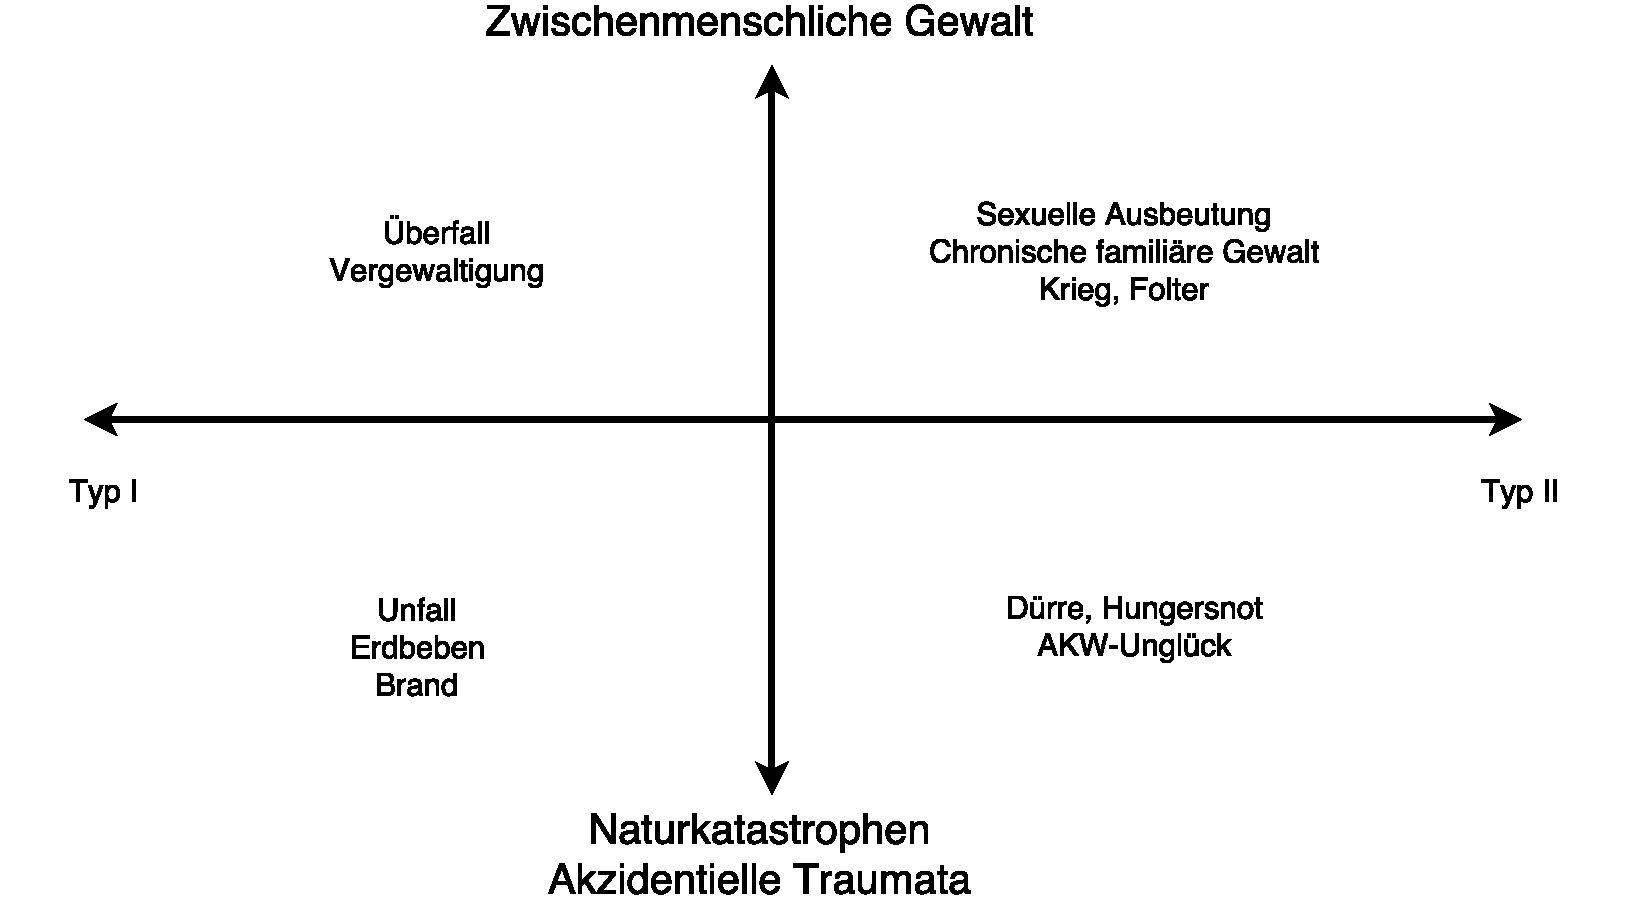
\includegraphics[scale=0.5]{abbildung1}
  \caption
      [Klassifikation traumatischer Ereignisse]
      {Klassifikation traumatischer Ereignisse (nach Landolt, 2004 zit. nach Landolt \& Hensel 2008: 14)}
\end{figure}

Die Entwicklung einer posttraumatischen Reaktion ist als Folge realer Erfahrungen und nicht als Eigenart des Individuums zu verstehen (vgl. Hensel 2014: 28).

\begin{quote}
\small{„Es sind die konkreten Lebensbedingungen, die psychische Symptome verursachen; es sind unbewältigte Lebenserfahrungen im Sinne einer Traumageschichte, die psychisch krank machen. Nur Störungen zu sehen, ohne den Hintergrund der Entstehung zu erkennen und anzuerkennen, bedeutet die Person zu pathologisieren.“ (Huber 2003: 31)}
\end{quote}

Diese Sichtweise ist keineswegs neu. Sie knüpft an die Anfänge der Psychotherapie (Psychoanalyse) und der freudschen Erkenntnis des Zusammenhangs zwischen der Erfahrung des sexuellen Missbrauchs in der frühen Kindheit und den Symptomen (Hysterie) im Erwachsenenalter an (vgl. Hensel 2014: 29 f.). Nach Freud ist ein Trauma „ein Erlebnis, welches dem Seelenleben innerhalb kurzer Zeit einen so starken Reizzuwachs bringt, dass die Erledigung oder Aufarbeitung derselben in normal-gewohnter Weise missglückt, woraus dauernde Störungen im Energiebetrieb resultieren müssen“ (Freud 1961: 284). 

\subsection{Traumapädagogik - Begriff und Definition}
Traumapädagogik wird als „Sammlungsbegriff für [...] Konzepte [benutzt], um die Handlungsfähigkeit der professionellen Fachkräfte wieder herzustellen und traumatisierten Kindern, Jugendlichen und Erwachsenen eine adäquate Teilhabe am sozialen Leben zu ermöglichen“ (Website Traumapädagogik o. J., vgl. Bausum u. a. 2013: 8). Aus den psychotraumatologischen Erkenntnissen sind, so Bausum, abgeleitete Konzeptionen entstanden, die in ihrer Komplexität als eigenständige „Fachrichtung der Traumapädagogik“ zu verstehen seien (ebd.).  

Der Begriff \textit{Traumapädagogik} bleibt schwammig und wird zum Teil unterschiedlich benutzt (vgl. Schmid u. a. 2007: 333). Der Begriff selbst ist vermutlich auf Volker Vogt und Martin Kühn zurückzuführen, die 2002 ein Webprojekt (www.traumapädagogik.de) als ein Diskussionsforum zur kindlichen Traumatisierung in der Pädagogik initiierten (vgl. Kühn 2006: 4; Weiß 2016b: 22). Kühn (2006: 5) distanzierte sich mit der Zeit von der anfangs als Arbeitstitel gedachten Bezeichnung seines Projektes. Der Name \textit{Traumapädagogik} zeige nicht deutlich genug, wozu und mit welchem Ziel gewirkt werden solle. Im Falle seines Konzeptes entscheidet er sich dafür, von einer \textit{Pädagogik} des sicheren Ortes zu sprechen (vgl. Kühn 2006: 4 f.). Kühn definiert Traumapädagogik als Ansatz zur Stabilisierung und Förderung traumatisierter Kinder und Jugendlicher. Sie sei eine notwendige Voraussetzung, Begleitung und Ergänzung eines entsprechenden Therapieprozesses. Daraus ergibt sich die Notwendigkeit eines engen interdisziplinären Austauschs und Diskurses zwischen Pädagogik, Psychotherapie und Psychiatrie (vgl. Kühn 2013: 27). Schmid versteht Traumapädagogik als „die konsequente Anwendung des aktuellen Kenntnisstands der Psychotraumatologie auf das pädagogische Verständnis der betreuten Menschen“ (Schmid 2013: 46). Damit meint er vor allem traumapädagogische Konzepte in der stationären Jugendhilfe als Beispiel für „die konsequente Umsetzung eines innovativen pädagogischen Konzepts, das auf klare psychopathologische Symptome abzielt“ (Schmid 2013: 57). Gemäß seinem Verständnis ist Traumapädagogik eine symptomspezifische, pädagogische Förderung psychisch belasteter Kinder und Jugendlicher (vgl. Schmid 2013: 57). Schmid u. a. (2007: 333) bemängeln, dass der Begriff häufig rein theoretisch besetzt werde, ohne daraus praktische Handlungskonsequenzen oder pädagogische Konzepte abzuleiten. Die Traumapädagogik entstand hauptsächlich an der Schnittstelle zwischen Kinder- und Jugendpsychiatrie/-psychotherapie und Jugendhilfe, die geholfen hat, „aus der Psychotraumatologie heraus milieutherapeutische Konzepte abzuleiten oder althergebrachte Konzepte der Heimerziehung aus einer psychotraumatologischen und neurobiologischen Perspektive heraus zu begründen“, so Schmid u. a. (2014: 174). Weiß (2016b: 29) sieht die Möglichkeit, die Haltungen und Methoden der Traumapädagogik vielseitig anzuwenden. Eine traumapädagogische Haltung sei eine solche, die für jede Pädagogik gültig sein sollte. Denn extremer Stress und traumatische Erfahrungen seien im Leben vieler Menschen verbreitet (vgl. ebd.). Weiß betont den Unterschied zwischen einerseits der Traumabearbeitung als der Bewältigung durch die Betroffenen und andererseits der Traumaarbeit, die die Begleitung durch psychosoziale Fachkräfte sei (vgl. Weiß 2016b: 20 f.). Sie versteht Traumapädagogik als notwendige Unterstützung traumatisierter Kinder und Jugendlicher im pädagogischen Alltag als Teil der Traumaarbeit (vgl. ebd.). Weiß u. a. definieren Traumapädagogik als eine junge Fachrichtung, die es sich zur Aufgabe gemacht hat, Fachkräfte, die mit traumatisch belasteten Kindern und Jugendlichen im Arbeitsalltag konfrontiert sind, zu unterstützen (vgl. Weiß u. a. 2016: 11). Dies soll durch spezifische Fort- und Weiterbildungen und die Schaffung tragfähiger Strukturen in den Institutionen geschehen (vgl. ebd.). Die Traumapädagogik sei als Antwort auf die Fragen der Praxis nach dem Umgang mit traumatisch belasteten Kindern und Jugendlichen in pädagogischen Arbeitsfeldern entstanden und fokussiere in der Auseinandersetzung mit dieser Frage drei Bereiche (vgl. Bausum u. a. 2013: 8):

\begin{itemize}
\item Begegnung zwischen Kind und pädagogischer Fachkraft 
\item Handlungssicherheit der pädagogischen Fachkraft 
\item Institutionelle Strukturen der Einrichtung
\end{itemize}

Die vorhandenen Definitionen der Traumapädagogik zeigen, dass diese noch ganz in den Anfängen steckt und anscheinend um ihre Berechtigung und Anwendungsbereiche kämpft. Die Traumapädagogik, trotz direkter Bezüge zur Psychotraumatologie, sagt nicht immer eindeutig aus, was unter Traumatisierung verstanden wird, was es wiederum erschwert, den Gegenstand und die Handlungsfelder zu bestimmen.

\subsection{Entstehung und Institutionalisierung der Traumapädagogik}
Die Anfänge der heute unter dem Begriff Traumapädagogik subsumierten Konzepte sind in stationären und teilstationären Einrichtungen der Kinder- und Jugendhilfe ab Mitte der 1990er-Jahre zu suchen (vgl. Weiß 2016b: 20). Ihnen vorausgegangen sind Ende der 1980er-Jahre Prozesse der Enttabuisierung des Themas sexueller Gewalt in der Kinder- und Jugendhilfe und folglich die Erweiterung des Blickwinkels auf andere Formen der Gewalt gegen Kinder. Stationäre Jugendhilfe, Pflegeeltern und Behindertenhilfe sind Bereiche, die Bedarf an entsprechenden Konzepten außerhalb des psychotherapeutischen Rahmens melden (vgl. Weiß 2016b: 20 f.).

Der Prozess der Professionalisierung und Institutionalisierung der Traumapädagogik beginnt zu Anfang dieses Jahrhunderts mit ersten Publikationen, Fort- und Weiterbildungen bis hin zur Gründung einer Bundesarbeitsgemeinschaft Traumapädagogik (BAG-TP), die sich zum Ziel setzt, das psychotraumatologische Wissen in verschiedene pädagogische Arbeitsfelder in Form von Diskussionen und Fortbildungen in traumabezogener Pädagogik zu tragen. Ihre Ziele sieht die BAG-TP in „Entwicklung, Förderung und Forschung von/zu Konzeptionen und Projekten in Erziehungs-, Bildungseinrichtungen und der Jugend-/Behindertenhilfe. Themen sind dabei u. a. die psychischen, physischen, sozialen und gesellschaftspolitischen Grundlagen und Folgen von Stressreaktionen bei Kindern und Jugendlichen auf traumatische Lebensereignisse und entsprechenden pädagogischen Begegnungen und Interventionsmöglichkeiten“ (BAG-TP 2011: 2). BAG-TP formuliert 2011 Traumapädagogische Standards in der stationären Kinder- und Jugendhilfe sowie, zusammen mit der Deutschsprachigen Gesellschaft für Psychotraumatologie (DeGPT), Kriterien für ein Curriculum Traumapädagogik/Traumazentrierte Fachberatung. Nach einer entsprechenden Weiterbildung, die momentan an 36 Instituten in Deutschland angeboten wird (vgl. DeGPT/Fachverband Traumapädagogik o. J.), kann eine Qualifikation für Traumapädagogik/Traumazentrierte Fachberatung erworben werden.

Hantke (2012: 198) beschreibt den Prozess der Entstehung der Traumapädagogik und ihrer Institutionalisierung vor dem Hintergrund der Ausdifferenzierung und Entgrenzung der therapeutischen, beraterischen und pädagogischen Bereiche. Die neuen Überlegungen, die aus der Traumatheorie resultieren, wurden in erste therapeutische Verfahren umgesetzt und diese dem Bereich der psychologischen Psychotherapie zugeschrieben. Damit sei der Zugang zu dem neuen Wissen und den Verfahren für viele psychosoziale Fachkräfte begrenzt gewesen. Die neuen, traumazentrierten Methoden, Denk- und Erklärungsansätze sollen Einzug in die stationäre Versorgung und in ambulante Settings in Form neu entstehender Traumapädagogik- und Traumaberatungscurricula gefunden haben (vgl. ebd.).

% !TeX encoding = UTF-8
\section{Traumap{\"a}dagogik - Haltung, Konzepte, traumasensible Organisationsentwicklung}

Traumapädagogik charakterisiert sich durch eine Grundhaltung, die als Basis des pädagogi-schen Handelns zu verstehen ist und sich in einem wertschätzenden pädagogischen Verständ-nis des Kindes zeigt (vgl. Schmied \& Lang 2012: 339). Aus den verschiedenen pädagogischen Konzepten, die zunächst aus der Praxis heraus entstanden sind, lassen sich handlungsleitende Inhalte herausarbeiten (vgl. Rothdeutsch-Granzer u. a. 2015: 178 f.). Traumapädagogik als konsequente Anwendung des psychotraumatologischen Wissens in der Ausgestaltung des pädagogischen Alltags und ein wertschätzendes Verständnis der betreuten Menschen berück-sichtigt alle Ebenen einer Organisation (vgl. Schmid \& Lang 2012: 339 ff.; BAG-TP 2011: 5) und kann als ein traumasensibler Organisationsentwicklungsprozess verstanden werden. Im Folgenden werden die traumapädagogische Haltung (2.1), wichtigste traumapädagische Kon-zepte und deren Inhalte (2.2) sowie die Traumap{\"a}dagogik als ein pädagogischs Konzept (3.3) fokussiert.

\subsection{Traumapädagogische Haltung}

Eine traumasensible Grundhaltung stellt die Basis für die Entwicklung traumapädagogischer Konzepte sowie eine Orientierung für das praktische und pädagogische Handeln dar (vgl. BAG-TP 2011: 4). Dabei soll das Wissen um die möglichen Folgen belastender Erlebnisse berücksichtigt werden, und es sollen die Ressourcen der Kinder und Jugendlichen im Mittel-punkt stehen (vgl. ebd.). Für die Entstehung der Traumap{\"a}dagogik seien Psychotraumatologie ebenso wie Soziale Arbeit, bindungstheoretische Grundlagen und Resilienzforschung, Neurobiologie und die therapeutischen Wissenschaften von Bedeutung (vgl. Weiß 2016b: 22). Traumap{\"a}dagogik beziehe sich auf Reformpädagogik, emanzipatorische Pädagogik und ver-trete das in der humanistischen Pädagogik und Psychologie begründete Menschenbild (vgl. Weiß 2016b: 23). Auf dieser Basis ist eine Reihe von Konzepten entstanden, die sich zwar in Inhalten und Gewichtung im pädagogischen Handeln unterscheiden, allerdings eine gemein-same Grundhaltung haben (vgl. ebd.). Die traumapädagogischen Standards formulieren dazu folgende fünf Handlungsansätze (vgl. BAG-TP 2011: 5 ff.):

\begin{itemize}
\item „Die Annahme des guten Grundes – Alles was ein Mensch zeigt, macht Sinn in seiner Geschichte!“ (ebd.: 5) 
\item „Wertsch{\"a}tzung – Es ist gut so, wie du bist!“ (ebd.: 5) 
\item „Partizipation – Ich traue dir was zu und {\"u}berfordere dich nicht!“ (ebd.: 6) 
\item „Transparenz – Jeder hat jederzeit ein Recht auf Klarheit!“ (ebd.: 6) 
\item „Spaß und Freude – Viel Freude tr{\"a}gt viel Belastung“ (ebd.: 7)
\end{itemize}

Im Zentrum der traumapädagogischen Haltung steht die Annahme des guten Grundes (vgl. Weiß 2016b: 23; Rothdeutsch-Granzer u. a. 2015: 177). Das Verhalten des Kindes wird dabei im Kontext seiner Biografie und Entwicklung als normale Reaktion auf eine außerordentliche Belastung verstanden. Das Kind soll in seinem Wesen und samt seinen Schwierigkeiten, die als Überlebensstrategien zu verstehen sind, angenommen und wertgeschätzt werden (vgl. ebd.). Transparenz im pädagogischen Alltag und die Teilhabe an der Gestaltung der eigenen Lebensbedingungen ermöglichen Kindern und Jugendlichen, Autonomie, Kompetenz und Zugeh{\"o}rigkeit zu erleben (vgl. BAG-TP 2011: 6). Dies sind wichtige Faktoren, die die seelische Gesundheit beeinflussen und eine Alternative zu den vorangegangenen Erfahrungen wie Gewalt, Vernachl{\"a}ssigung und/oder Missbrauch anbieten. Spaß und Freude zu erleben, wirkt ausgleichend zu den belastenden Erlebnissen, die die Gefühlswelt in ein Ungleichgewicht bringen (vgl. ebd.). Die traumapädagogische Haltung solle nicht nur den Kindern und Jugendlichen gegenüber gelten, sondern die MitarbeiterInnen und KooperationspartnerInnen miteinschließen (vgl. Schmid \& Lang 2012: 345).

\subsection{Traumapädagogische Konzepte – handlungsleitende Inhalte}
Traumapädagogik als Sammlung von Konzepten, die traumatisierte Mädchen und Jungen sowie junge Erwachsene im pädagogischen Alltag unterstützen, ist aus der pädagogischen Praxis entstanden. Diese Konzepte weisen einige Gemeinsamkeiten auf, vor allem in Bezug auf die Grundhaltung (siehe 2.1), als auch Unterschiede in Inhalten und im Handeln (vgl. Weiß 2016b: 23). Aus diesen Konzepten lassen sich handlungsleitende Inhalte für das pädagogische Handeln herausarbeiten (vgl. Rothdeutsch-Granzer u. a., 2015: 178 f.; siehe Abbildung \ref{fig:inhalte})

\begin{figure}[h]
  \centering
  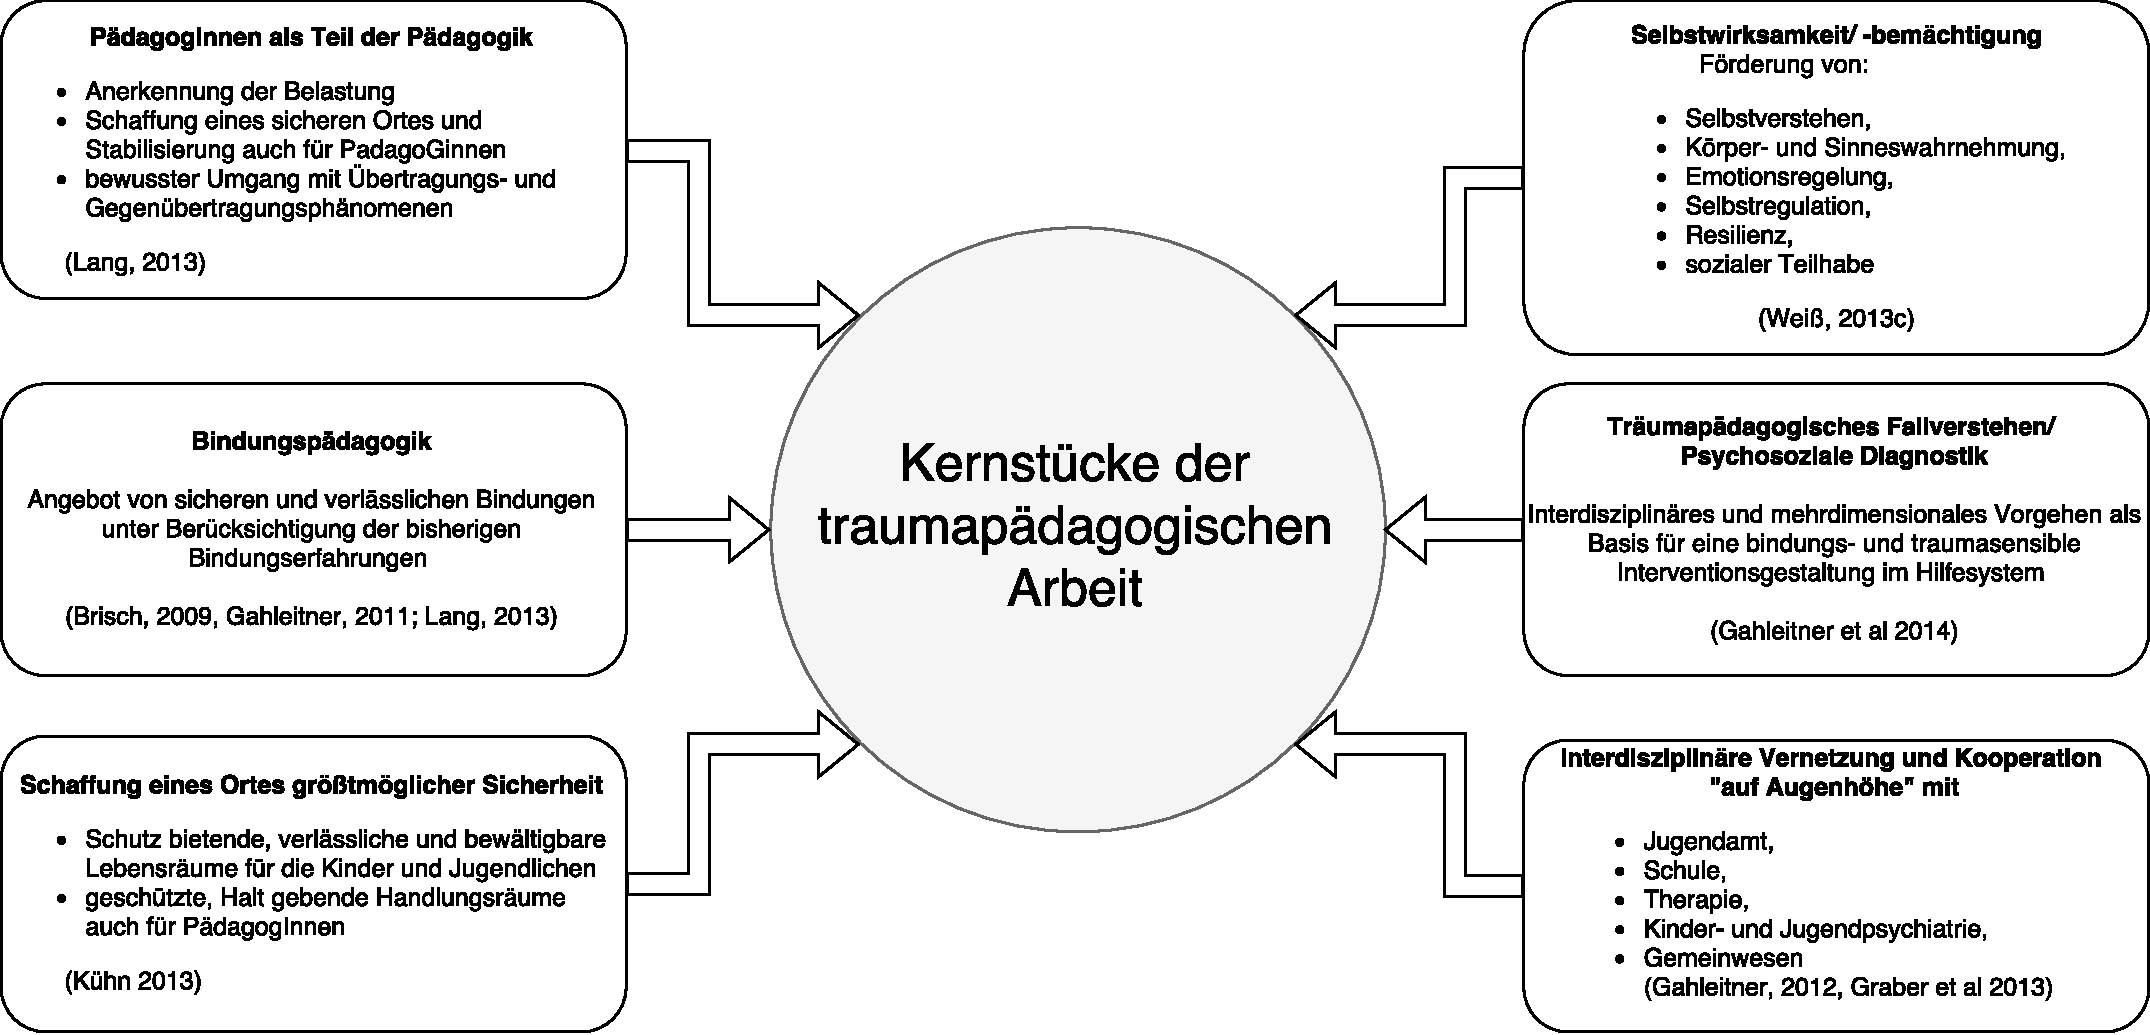
\includegraphics[scale=0.45]{abbildung2}
  \caption
      [Handlungsleitende Inhalte der traumapädagogischen Arbeit]
      {Handlungsleitende Inhalte der traumapädagogischen Arbeit (nach Rothdeutsch-Granzer u. a., 2015: 179)}
  \label{fig:inhalte}
\end{figure}

Kühn (2014: 21) bezeichnet drei Kernkonzepte als richtungsweisend in der Traumap{\"a}dagogik: \textit{Pädagogik des sicheren Ortes} (vgl. Kühn 2006), \textit{Traumazentrierte Pädagogik} nach Uttendörfer (2008) und \textit{Pädagogik der Selbstbemächtigung} nach Weiß (2016a). Mittlerweile sind weitere Konzepte und Anwendungen entstanden, die die Vielfältigkeit der Handlungsfelder zeigen, in denen psychotraumatologisches Wissen gefragt ist. Das sind, um einige Beispiele zu nennen: \textit{Traumapädagogische Gruppenarbeit} nach Bausum (2013), \textit{Stabilisierung und (Selbst-)Fürsorge für PädagogInnen} (Lang 2013), \textit{Traumapädagogik in der Schule} (Ding 2013, Zimmerman 2016) und \textit{Milieutherapeutische Konzepte} (Gahleitner 2011). Auch in weiteren Handlungsfeldern und für AdressatInnen wie z. B. Ehe- und Familienberatung, Gefangenenseelsorge, Gewaltprävention, Frauenhäuser, Wohneinrichtungen für unbegleitete minderjährige Flüchtlinge etc. sei traumapädagogisches Wissen gefragt (vgl. Hantke 2015: 118).  

Die gemeinsamen Inhalte der Konzepte sind in Bezug auf den \textit{sicheren Ort} und die Bedeutung der Bindung sowie positiver Beziehungserfahrungen für die Traumabearbeitung am weitesten entwickelt (vgl. Weiß 2016b: 27). Viele Konzepte adaptieren (psycho-)therapeutische Methoden, um z. B. mit Fertigkeitstrainings oder Notfallkoffern die Emotionsregulation zu begleiten (vgl. ebd.: 28). Einige Konzepte betonen die Wichtigkeit und Bedeutung der traumatischen Übertragungs- und Gegenübertragungsreaktionen (vgl. Kessler 2016: 123 ff.; Schmid 2013: 48) und formulieren entsprechende Interventionen. Die Traumabearbeitung als ein Prozess der Selbstbemächtigung nach Weiß (2016b: 20) beinhaltet unter anderem: traumabedingte Einstellungen und Überzeugungen zu verändern; das Geschehen in die eigene Lebensgeschichte einzuordnen; die Möglichkeit, in der Gegenwart Sinn zu finden; Körperfürsorge und Körpergewahrsein zu entwickeln; Selbstregulation zu erlernen; die traumatischen Erinnerungen und den traumatischen Stress zu kontrollieren sowie soziale Teilhabe zu ermöglichen. Dieses Konzept betont vor allem die Expertenschaft der Kinder und Jugendlichen. Ihnen soll das Wissen über Traumatisierung zur Verfügung gestellt werden (vgl. ebd.).  

Schmid und Lang (2012: 347) sehen Psychoedukation als bedeutenden Bestandteil der Traumap{\"a}dagogik. Ziel sei es, den Kindern und Jugendlichen ihre Reaktionen und Symptome, neurobiologische Abl{\"a}ufe, das Entstehen von Spannungszust{\"a}nden, K{\"o}rperreaktionen und Dissoziationen\footnote{Das Einstellen der Aussenwahrnehmung und ein tranceartiger Zustand, begleitet von einem Verlust des Körpers und Zeitgefühls, der räumlichen Orientierung, der Schmerzwahrnehmung, oft mit einem Derealisationserleben verbunden (vgl. Schmid u. a. 2010; 49 f.). Gefühle und Gedanken werden getrennt und im Falle der Traumatisierung kann ein Verlust der Integration der Erinnerungen an die Vergangenheit eintreten (vgl. Weiß u. a. 2016; 460).} etc. in einer altersangemmessenen und verständlichen Form mit bildhafter Sprache und grafischer Unterstützung zu erklären. Dabei sei die Botschaft wichtig, dass Symptome und Schwierigkeiten der Heranwachsenden eine normale, menschliche Reaktion auf v{\"o}llig unnormale und unmenschlichet Erlebnisse darstellen. Wichtig sei es, dass das Kind und die mit ihm arbeitenden Erwachsenen die gleiche Terminologie benutzten, um eine gemeinsame Sprache für spätere Interventionen und Analyse von schwierigen Situationen zu entwickeln (vgl. Schmid \& Lang 2012: 347).

\subsection{Traumapädagogik als Konzept}
Die BAG-TP sieht die Notwendigkeit, die Erkenntnisse der Psychotraumatologie und der Hirnforschung in den Institutionen, in denen traumatisierte Mädchen und Jungen betreut werden, umzusetzen (vgl. BAG-TP 2011: 4 f.). Klare Haltungen, F{\"o}rderans{\"a}tze und Methoden, die in der Umsetzung traumap{\"a}dagogischer Konzepte unerl{\"a}sslich seien, bilden die Grundlage f{\"u}r die von der BAG-TP formulierten Standards zur traumap{\"a}dagogischen Arbeit in Einrichtungen der station{\"a}ren Kinder- und Jugendhilfe. Im Mittelpunkt eines traumapädagogischen Konzepts steht laut der BAG-TP, verlässliche Beziehungen im Alltag aufzubauen und zu gewährleisten, die Traumatisierten sozial und emotional zu stabilisieren sowie das Selbstvertrauen der zu betreuenden Kindern und Jugendlichen aufzubauen und zu stärken (vgl. ebd.). Dabei soll die traumapädagogische Grundhaltung (siehe 2.1) als Voraussetzung institutionell durchg{\"a}ngig erkennbar bleiben (vgl. BAG-TP 2011: 5 ff.). Eine Einrichtung, die traumapädagogisch arbeitet, soll zu einem sicheren Ort werden, an dem betroffene Kinder und Jugendliche „neue, erg{\"a}nzende Erfahrungen machen k{\"o}nnen, sich selbst und ihre Handlungsstrategien verstehen lernen, Entwicklungshemmnisse aufholen und sichere Bindungserfahrungen machen k{\"o}nnen“ (BAG-TP 2011: 4). Die Entwicklung dieses Ortes soll alle Beteiligten mit einbeziehen und als ein institutioneller und kontinuierlicher Prozess verstanden werden. Die Einführung eines traumapädagogischen Konzepts im Sinne eines sicheren Ortes soll mehrere Ebenen einer Institution miteinschließen (vgl. ebd.). Schmid (2013: 49) versteht das Einbeziehen der MitarbeiterInnen und der strukturellen Abläufe in die (trauma-)pädagogische Konzeption als zentral. Um den Kindern und Jugendlichen einen stabilisierenden, sicheren Rahmen zu bieten, bedarf es solcher MitarbeiterInnen und Strukturen, die selbst stabil und selbstwirksam sind. Die MitarbeiterInnen und Teams brauchen, um bei den Krisen stabilisierend zu wirken, dieselben Fertigkeiten wie die Kinder und Jugendlichen selbst (vgl. ebd.). Schmid (2013: 49) beschreibt eine Institution, die ein traumapädagogisches Konzept umsetzt, als eine Versorgungskette, am Anfang derer das Kind steht, das im Alltag unterstützt werden soll (siehe Abbildung \ref{fig:konzept}). Hierzu bedarf es jedoch stabiler und stabilisierender Strukturen auf allen Ebenen der Organisation (vgl. ebd.).

\begin{figure}[h]
  \centering
  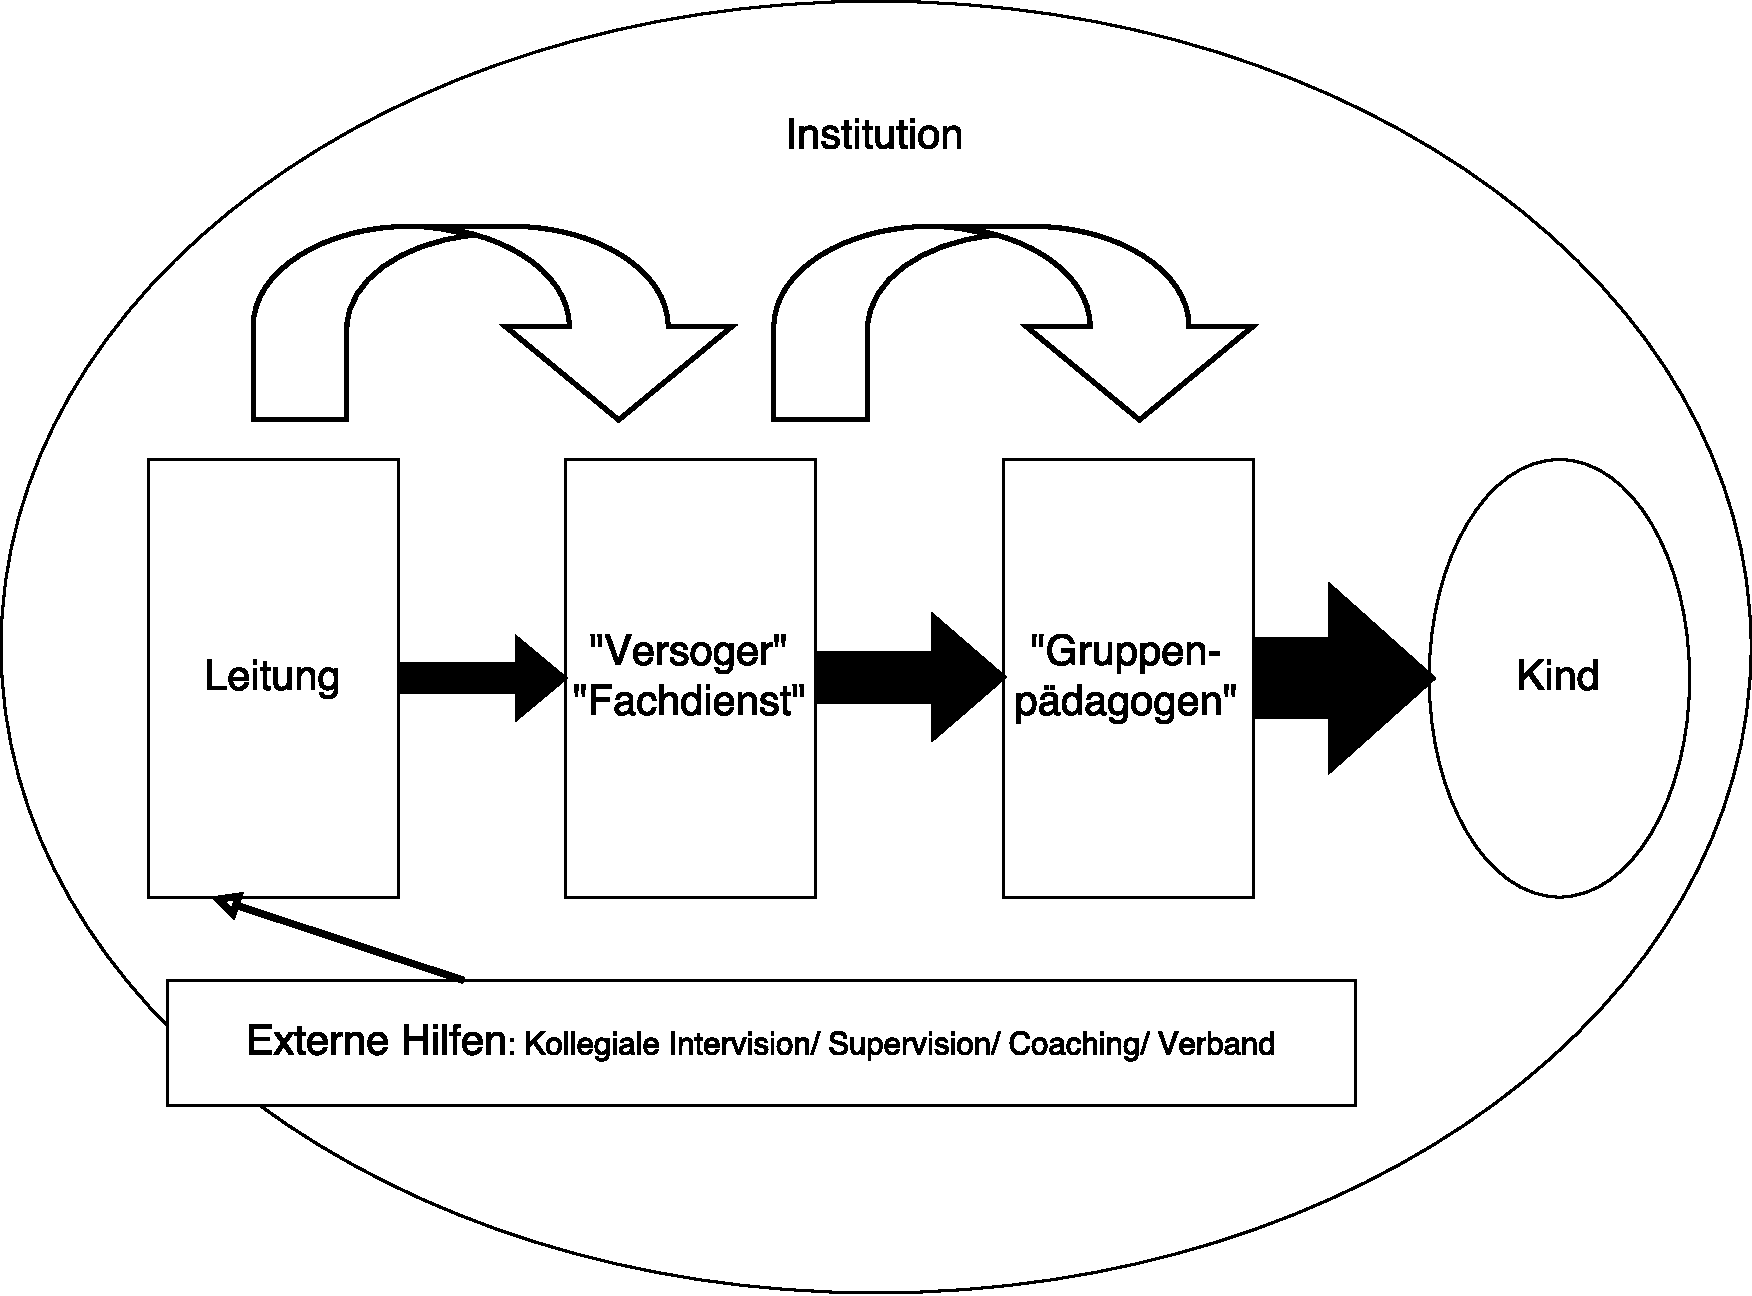
\includegraphics[scale=0.3]{abbildung3}
  \caption
      [Konzept einer Versorgungskette]
      {Konzept einer Versorgungskette (nach Schmid 2013: 49)}
  \label{fig:konzept}
\end{figure}

Traumap{\"a}dagogik sowie traumapädagogische Standards können laut Schirmer (2016: 443 f.) als Paradigmenwechsel in der Heimerziehung gewertet werden. Dieser besteht darin, dass die pädagogischen Fachkräfte, Kinder und Jugendlichen und die institutionellen Strukturen in das pädagogische Konzept im Sinne einer wertgeleiteten Organisations- und Personalentwicklung mit der zugrunde liegenden wertschätzenden verstehender Grundhaltung einbezogen werden. Diese Haltung richtet sich darauf, das „unerwünschte“ Verhalten reflexiv zu verstehen und gemeinsam nach Lösungen und pädagogisch nachvollziehbaren pädagogischen Interventionen zu suchen (vgl. ebd.).


\clearpage
\setcounter{secnumdepth}{0}
% !TeX encoding = UTF-8
\section{Literaturverzeichnis}

\setlength{\parindent}{0pt}
\hang
Anhorn, R. \& Balzereit, M. (2016). Die »Arbeit am Sozialen« als »Arbeit am Selbst« - Herrschaft, Soziale Arbeit und die therapeutische Regierungsweise im Neo-Liberalismus: Einf{\"u}hrende Skizzierung eines Theorie- und Forschungsprogramms. In R. Anhorn \& M. Balzereit (Hrsg.), \textit{Handbuch Therapeutisierung und Soziale Arbeit} (S. 3-207). Wiesbaden: Springer.

\hang
Bausum, J. (2013). Ressourcen der Gruppe zur Selbstbem{\"a}chtigung. „Ich bin und ich brauche euch". In J. Bausum, L. U. Bessr, M. Kühn \& W. Weiß (Hrsg.), \textit{Traumapädagogik: Grundlagen}, \textit{Arbeitsfelder und Methoden für die pädagogische Praxis} (S. 179-188). Weinheim: Beltz.

\hang
Bausum, J., Bessr, L. U., Kühn, M. \& Weiß, W. (Hrsg.). (2013). \textit{Traumapädagogik: Grundlagen, Arbeitsfelder und Methoden für die pädagogische Praxis.} Weinheim: Beltz.

\hang
Becker, D. (2006). \textit{Die Erfindung des Traumas: verflochtene Geschichten}. Gießen: Psychosozial.

\hang
Bundesarbeitsgemeinschaft Traumap{\"a}dagogik – BAG-TP (2011). \textit{Standards für traumapädagogische Konzepte in der stationären Kinder- und Jugendhilfe.} Gnarrenburg: BAG-Traumapädagogik. Verfügbar unter: http://www.bag-traumapaedagogik.de/index.php/standards.html\break[22.03.2017].

\hang
Bundesministerium für Familie, Senioren, Frauen und Jugend – BMFSFJ (2009). \textit{13. Kinder- und Jugendbericht Bericht über die Lebenssituation junger Menschen und die Leistungen der Kinder- und Jugendhilfe.} Berlin. Verfügbar unter:\\ https://www.bmfsfj.de/blob/93144/f5f2144cfc504efbc6574af8a1f30455/13-kinder-jugend-bericht-data.pdf [25.04.2017].

\hang
Ding, U. (2013). Trauma und Schule. Was l{\"a}sst Peter wieder lernen? {\"U}ber unsichere Bedingungen und sichere Orte in der Schule. In J. Bausum, L. U. Bessr, M. Kühn \& W. Weiß (Hrsg.), \textit{Traumapädagogik: Grundlagen, Arbeitsfelder und Methoden für die pädagogische Praxis} (S. 55-66). Weinheim: Beltz.

\hang
Fachverband Traumapädagogik - DeGPT (o. J.). \textit{Anerkannte Ausbildungsinstitute für Traumapädagogik und Traumazentrierte Fachberatung.} Verfügbar unter: http://www.degpt.de/DeGPT-Dateien/Institute-Traumap\%C3\%A4dagogik-April\%202017.pdf [08.05.2017].

\hang
Falkai, P., Wittchen, H.-U. \& American Psychiatric Association (APA). (2015). \textit{Diagnostisches und statistisches Manual psychischer Störungen DSM-5 / American Psychiatric Association; Deutsche Ausgabe.} G{\"o}ttingen: Hogrefe.

\hang
Fegert, J. M., Ziegenhain, U. \& Goldbeck, L. (Hrsg.). (2013). \textit{Traumatisierte Kinder und Jugendliche in Deutschland Analysen und Empfehlungen zu Versorgung und Betreuung.} Weinheim: Beltz.

\hang
Freud, S. (1961). \textit{Gesammelte Werke. 11, Vorlesungen zur Einführung in die Psychoanalyse.} Fischer Verlag: Frankfurt am Main.

\hang
Gahleitner, S. B. (2011). \textit{Das Therapeutische Milieu in der Arbeit mit Kindern und Jugendlichen: Trauma- und Beziehungsarbeit in stationären Einrichtungen.} Bonn: Psychiatrie-Verlag.

\hang
Gahleitner, S. B. \& Homfeld, H. G. (2016). Kooperation und psychosoziale Traumaarbeit. In W. Weiß, T. Kessler \& S. B. Gahleitner (Hrsg.), \textit{Handbuch Traumapädagogik} (S. 320-326). Weinheim: Beltz.

\hang
Hantke, L. (2012). Traumazentrierte Arbeit im psychosozialen Feld. Unterschiede und Gemeinsamkeiten von Traumatherapie, -beratung und -pädagogik. In \textit{Trauma \& Gewalt, 3} (6), 198-205. Stuttgart: Klett-Cotta.

\hang
Hantke, L. (2015). Traumakompetenz in psychosozialen Handlungsfeldern. In S. B. Gahleitner, C. Frank \& A. Leitner (Hrsg.), \textit{Ein Trauma ist mehr als ein Trauma : biopsychosoziale Traumakonzepte in Psychotherapie, Beratung, Supervision und Traumapädagogik} (S. 118-126). Weinheim: Beltz.

\hang
Hantke, L. \& Görges, H. (2012). \textit{Handbuch Traumakompetenz: Basiswissen für Therapie, Beratung und Pädagogik.} Paderborn: Junfermann.

\hang
Hausmann, C. (2006). \textit{Einführung in die Psychotraumatologie.} Wien: Facultas.

\hang
Hensel, T. (2013). Traumatherapie bei Kindern und Jugendlichen. Ausbildungs- und Versorgungsrealit{\"a}t aus der Sicht eines niedergelassenen Kinder- und Jugendlichenpsychotherapeuten und Ausbilders in Kindertraumapsychotherapie. In J. M. Fegert, U. Ziegenhain \& L. Goldbeck (Hrsg.), \textit{Traumatisierte Kinder und Jugendliche in Deutschland.} Analysen und Empfehlungen zu Versorgung und Betreuung (S. 82-88).Weinheim: Beltz.

\hang
Hensel, T. (2014). Die Psychotraumatologie des Kindes- und Jugendalters. In S. Gahleitner, T. Hensel, M. Baierl, M. K{\"u}hn \& M. Schmid (Hrsg.), \textit{Traumap{\"a}dagogik in psychosozialen Handlungsfeldern. Ein Handbuch f{\"u}r Jugendhilfe, Schule und Klinik} (S. 27-40). Göttingen: Vandenhoeck \& Ruprecht.

\hang
Huber, M. (2003). \textit{Trauma und Traumabehandlung. 1. Trauma und die Folgen.} Paderborn: Junfermann.

\hang
ICD-10-GM. (2016). \textit{Die Internationale statistische Klassifikation der Krankheiten und verwandter Gesundheitsprobleme, 10. Revision, German Modification.} Verfügbar unter:\\ https://www.dimdi.de/static/de/klassi/icd-10-gm/kodesuche/onlinefassungen\\
/htmlgm2016/block-f40-f48.htm [23.01.2017].

\hang
Kessler, T. (2016). {\"A}ußere Eindr{\"u}cke und innere Erwartungen. Theoretische Aspekte zu den Dynamiken von {\"U}bertragung und Gegenreaktion in der traumap{\"a}dagogischen Arbeit. In W. Weiß, T. Kessler \& S. B. Gahleitner (Hrsg.), \textit{Handbuch Traumapädagogik} (S. 123-130). Weinheim: Beltz.

\hang
Kühn, M. (2006). \textit{Bausteine einer „P{\"a}dagogik des Sicheren Ortes“ - Aspekte eines p{\"a}dagogischen Umgangs mit (traumatisierten) Kindern in der Jugendhilfe aus der Praxis des SOS-Kinderdorfes Worpswede.} Vortrag: Fachtagung „(Akut) traumatisierte Kinder und Jugendliche in P{\"a}dagogik und Jugendhilfe“. Merseburg, 17./18.02.2006. Verfügbar unter:\\ http://www.jugendsozialarbeit.de/media/raw/martin\_kuehn.pdf [24.02.2017].

\hang
Kühn, M. (2013). Macht eure Welt endlich wieder mit zu meiner. Anmerkungen zum Begriff der Traumapädagogik. In J. Bausum, L. U. Besser, M. Kühn \& W. Weiß (Hrsg.), \textit{Traumapädagogik: Grundlagen, Arbeitsfelder und Methoden für die pädagogische Praxis} (S. 24-37). Weinheim: Beltz.

\hang
Kühn, M. (2014). Traumap{\"a}dagogik - von einer Graswurzelbewegung zur Fachdisziplin. In S. Gahleitner, T. Hensel, M. Baierl, M. K{\"u}hn \& M. Schmid (Hrsg.), \textit{Traumap{\"a}dagogik in psychosozialen Handlungsfeldern. Ein Handbuch f{\"u}r Jugendhilfe, Schule und Klinik} (S. 21-26). Göttingen: Vandenhoeck \& Ruprecht.

\hang
K{\"u}hner, A. (2005). Schmerzfreier {\"u}ber Leiden sprechen? Gedankenexperimente und Beobachtungen zu Ambivalenzen des Traumabegriffs. In A. Karger \& R. Heinz (Hrsg.), \textit{Trauma und Schmerz. Psychoanalytische, philosophische und sozialwissenschaftliche Perspektiven} (S. 165-172). Gießen: Psychosozial.

\hang
Landolt, M. \& Hensel, T. (Hrsg.). (2008). \textit{Traumatherapie bei Kindern und Jugendlichen.} Göttingen: Hogrefe.

\hang
Lang, B. (2013). Stabilisierung und (Selbst-) F{\"u}rsorge f{\"u}r p{\"a}dagogische Fachkr{\"a}fte als institutioneller Auftrag. In J. Bausum, L. U. Besser, M. Kühn \& W. Weiß (Hrsg.), \textit{Traumapädagogik: Grundlagen, Arbeitsfelder und Methoden für die pädagogische Praxis} (S. 211-220). Weinheim: Beltz.

\hang
Maercker A. (Hrsg.). (2009). \textit{Posttraumatische Belastungsst{\"o}rungen.} Heidelberg: Springer.

\hang
M{\"o}hrlein, G. \& Hoffart, E.-M. (2014). Traumap{\"a}dagogische Konzepte in der Schule. In S. B. Gahleitner, T. Hensel, M. Baierl, M. K{\"u}hn \& M. Schmid (Hrsg.), \textit{Traumap{\"a}dagogik in psychosozialen Handlungsfeldern. Ein Handbuch f{\"u}r Jugendhilfe, Schule und Klinik} (S. 91-103). Göttingen: Vandenhoeck \& Ruprecht.

\hang
Purtscher-Penz, K. (2015). Traumatisierung in der Kindheit und Jugend. Hilfe durch Psychotherapie und Traumap{\"a}dagogik. In S. B. Gahleitner, Ch. Frank, \& A. Leitner (Hrsg.), \textit{Ein Trauma ist mehr als ein Trauma : biopsychosoziale Traumakonzepte in Psychotherapie, Beratung, Supervision und Traumap{\"a}dagogik} (S. 95-105). Weinheim: Beltz.

\hang
Reinelt, T., Vasileva, M. \& Petermann, F. (2016). Psychische Auff{\"a}lligkeiten von Fl{\"u}chtlingskindern: Eine Blickverengung durch die Posttraumatische Belastungsst{\"o}rung? \textit{Kindheit und Entwicklung}, 25(4), 231-237.

\hang
Rothdeutsch-Granzer, Ch., Weiß, W. \& Gahleitner, S. B. (2015). Traumap{\"a}dagogik – eine junge Fachrichtung mit traditionsreichen Wurzeln und hoffnungsvollen Perspektiven. In S. B. Gahleitner, C. Frank \& A. Leitner (Hrsg.), \textit{Ein Trauma ist mehr als ein Trauma: biopsychosoziale Traumakonzepte in Psychotherapie, Beratung, Supervision und Traumap{\"a}dagogik} (S. 171-186). Weinheim: Beltz.

\hang
Saß, H., Wittchen, H. U., Zaudig, M. \& Houben, I. (2003). \textit{Diagnostisches und Statistisches Manual Psychischer Störungen – Textrevision – DSM-IV-TR.} Göttingen: Hogrefe.

\hang
Schirmer, C. (2016). Die Entwicklung der traumapädagogischen Standards. Ein Meilenstein in der stationären Erziehungshilfe. In W. Weiß, T. Kessler \& S. B. Gahleitner (Hrsg.), \textit{Handbuch Traumapädagogik} (S.439-448). Weinheim: Beltz.

\hang
Schmid, M. (2013). Umgang mit traumatisierten Kindern und Jugendlichen in der station{\"a}ren Jugendhilfe: „Traumasensibilit{\"a}t“ und „Traumap{\"a}dagogik“. In J. M. Fegert, U. Ziegenhain \& L. Goldbeck (Hrsg.), \textit{Traumatisierte Kinder und Jugendliche in Deutschland Analysen und Empfehlungen zu Versorgung und Betreuung} (S. 36-60). Weinheim: Beltz.

\hang
Schmid, M. \& Lang, B. (2012). Was ist das Innovative und Neue an einer Traumap{\"a}dagogik? In M. Schmid, M. Tetzer, K. Rensch \& S. Schlüter- Müller (Hrsg.), \textit{Handbuch Psychiatriebezogene Sozialpädagogik} (S. 337-351). Göttingen: Vandenhoeck \& Ruprecht.

\hang
Schmid, M., Fegert, J. M. \& Petermann, F. (2010). Traumaentwicklungsstörung: Pro und Contra. \textit{Kindheit und Entwicklung, 19} (1), 47-63.

\hang
Schmid, M., Purtscher-Penz, K., Stellermann-Strehlow, K. (2014). Traumasensibilit{\"a}t und traumap{\"a}dagogische Konzepte in der Kinder- und Jugendpsychiatrie/-psychotherapie. In S. B. Gahleitner, T. Hensel, M. Baierl, M. K{\"u}hn \& M. Schmid (Hrsg.), \textit{Traumap{\"a}dagogik in psychosozialen Handlungsfeldern Ein Handbuch f{\"u}r Jugendhilfe, Schule und Klinik} (S. 174-191). Göttingen: Vandenhoeck \& Ruprecht.

\hang
Schmid, M.,Wiesinger, D., Lang, B., Jaszkowic, K. \& Fegert, J. M. (2007). Brauchen wir eine Traumap{\"a}dagogik? – Ein Pl{\"a}doyer f{\"u}r die Entwicklung und Evaluation von traumap{\"a}dagogischen Handlungskonzepten in der station{\"a}ren Jugendhilfe. \textit{KONTEXT} 38(4), 330-357.

\hang
Strauß, J.W. (2016). Grenzen der Traumap{\"a}dagogik – kritische (Nach-)Fragen. In W. Weiß, T. Kessler \& S. B. Gahleitner (Hrsg.), \textit{Handbuch Traumapädagogik} (S. 449-457). Weinheim: Beltz.

\hang
Uttendörfer, J. (2008). Traumazentrierte Pädagogik. Von der Entwicklung der Kultur eines „Sicheren Ortes“. \textit{Unsere Jugend}, 60(2), 50-6.

\hang
Website Traumapädagogik (o. J.). Herzlich Willkommen. Verfügbar unter:\\ http://www.traumapaedagogik.de/[08.05.2017].

\hang
Weiß, W. (2003). \textit{Philipp sucht sein Ich: Zum pädagogischen Umgang mit Traumata in den Erziehungshilfen} (1. Aufl.). Weinheim: Votum.

\hang
Weiß, W. (2013). \textit{Philipp sucht sein Ich: Zum pädagogischen Umgang mit Traumata in den Erziehungshilfen} (7. Aufl.). Weinheim: Juventa.

\hang
Weiß, W. (2016a). Die Pädagogik der Selbstbemächtigung. Eine traumapädagogische Methode. In W. Weiß, T. Kessler \& S. B. Gahleitner (Hrsg.), \textit{Handbuch Traumapädagogik} (S. 290-302). Weinheim: Beltz.

\hang
Weiß, W. (2016b). Traumap{\"a}dagogik: Entstehung, Inspirationen, Konzepte. In W. Weiß, T. Kessler \& S. B. Gahleitner (Hrsg.), \textit{Handbuch Traumapädagogik} (S. 20-32). Weinheim: Beltz.

\hang
Weiß, W., Kessler, T. \& Gahleitner, S. B. (Hrsg.). (2016). \textit{Handbuch Traumapädagogik.} Weinheim: Beltz.

\hang
Zimmermann, D. (2016). \textit{Traumapädagogik in der Schule: Pädagogische Beziehungen mit schwer belasteten Kindern und Jugendlichen.} Gießen: Psychosozial-Verlag.


\setcounter{secnumdepth}{2}
\appendix
% !TeX encoding = UTF-8
\section{Anhang}
\vspace{6cm}
Name: Urbaniak \hfill Vorname: Olga \hfill Matrikelnr.: 4802822
\section*{Eidesstattliche Erklärung zur Bachelorarbeit}
Ich versichere, die Bachelorarbeit selbstständig und lediglich unter Benutzung der angegebenen Quellen und Hilfsmittel verfasst zu haben.
\\\\
Ich erkläre weiterhin, dass die vorliegende Arbeit noch nicht im Rahmen eines anderen Prüfungsverfahrens eingereicht wurde.
\\\\
Berlin, den \thesisDate
\clearpage
\pagestyle{fancy}
\fancyhf{} %alle Kopf- und Fußzeilenfelder bereinigen


\end{document}
